多くの低レイヤのネットワークアプリケーションの開発者の目には一切のプログラムがどれもSocketのように映ります。すこし大げさかもしれませんが、だいたいこのようなものです。現在のネットワークプログラミングはほぼすべてにおいてSocketを使用してプログラムされています。このような場面を考えたことはありませんか?毎日ブラウザを開いてページを閲覧する際、ブラウザプロセスはどのようにしてWebサーバと通信を行っているのでしょう?QQを使ってチャットする時、QQプロセスはどのようにしてサーバまたはあなたの友達がいるQQプロセスと通信を行なっているのでしょう?PPstreamを開いてストリーミング映像を見るとき、PPstreamプロセスはどのようにして動画サーバと通信を行っているのでしょう?このように、すべてはSocketに依存して通信を行なっています。ひとつを見てすべてを理解すると、Socketプログラミングは現代のプログラミングの中でも非常に多くの重要な地位を占めていることが見て取れます。この章ではGo言語においてどのようにSocketプログラミングを行うのかご紹介します。

\subsubsection{Socketとは何か?}
SocketはUnixを起源とします。Unixの基本哲学の一つは"すべてはファイルである"です。すべては"開くopen -$>$ 読み書きwrite/read -$>$ 閉じるclose"のパターンによって操作されます。Socketはこのパターンの実装の一つです。ネットワークのSocketデータ通信は特殊なI/Oの一つです。Socketもファイルディスクリプタの一種です。Socketもファイルを開く関数を持っています:Socket()。この関数はint型のSocketディスクリプタを返します。以後の接続の確立によってデータ転送といった操作はすべてこのSocketを通ることで実現されます。

よく使われるSocketには二種類があります:ストリームSocket(SOCK\_STREAM)とデータグラムSocket(SOCK\_DGRAM)です。ストリームは接続指向のSocketの一種です。接続指向のTCPサービスアプリケーションに使用されます。またデータグラムSocketは無接続のSocketの一種です。接続の無いUDPサービスアプリケーションに利用されます。

\subsubsection{Socketはどのようにして通信を行うか}
ネットワークではプロセス間はどのようにしてSocketを使って通信を行うのでしょうか?まず解決しなければならない問題はどのようにユニークなプロセスのひとつを認識するのかということです。そうでなければ通信を始めることすらままなりません!ローカルでプロセスPIDを使って一つのプロセスを識別します。実はTCP/IPプロトコル族ではすでにこの問題を解決してくれています。ネットワーク層の"ipアドレス"はネットワーク上のホストを一意に認識しており、トランスポート層の"プロトコル+ポート"はホストのアプリケーションプログラム(プロセス)を一意に認識することができます。これら3つの組み合わせ(ipアドレス、プロトコル、ポート)を利用することで、ネットワークのプロセスを認識することができます。ネットワークにおいて通信を行う必要のあるプロセスはこのタグを利用して互い通信を行うことができます。以下のTCP/IPプロトコルの構造図をご覧ください。

\begin{figure}[H]
  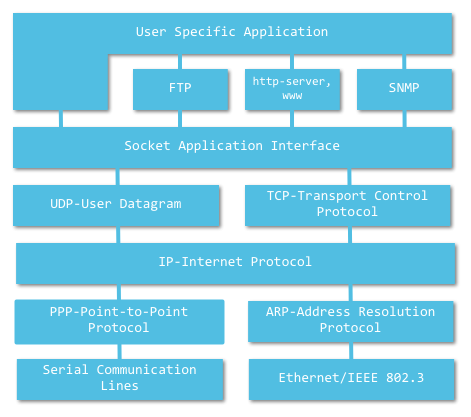
\includegraphics[width=14cm]{8.1.socket.png}
   \label{図8.1}
   \caption{七階層のネットワークプロトコルの図}
\end{figure}

TCP/IPプロトコルを使用したアプリケーションプログラムは通常アプリケーションプログラムのポートを採用します:UNIX BSDのソケット(socket)とUNIX System VのTLI(すでに淘汰されています)によってネットワークプロセス間の通信を実現します。現在ではほぼすべてのアプリケーションプログラムではsocketが採用されています。現在はネットワーク時代で、ネットワークのプロセス通信はどこにでも存在します。"すべてがSocket"というのはこういうことです。

\subsubsection{Socketの基礎知識}
Socketには二種類存在することをご紹介しました:TCP SocketとUDP Socketです。TCPとUDPはプロトコルで、ひとつのプロセスを確定するためには3つの組が必要です。IPアドレスとポート番号が必要です。

\paragraph{IPv4アドレス}
現在のインターネットが採用しているプロトコル族はTCP/IPプロトコルです。IPはTCP/IPプロトコルのネットワーク層のプロトコルです。TCP/IPプロトコル族のコアとなるプロトコルです。現在主に採用されているIPプロトコルのバージョンは4(簡単な呼び名はIPv4)です。現在まで30数年あまりに渡って使用されてきました。

IPv4のアドレスビット数は32ビットです。つまり多くても2の32乗のネットワーク機器がInternetに接続できることになります。ここ十年来インターネットの力強い発展にともなって、IPアドレスの需要は高まりつつあります。IPアドレスの割り当てはより厳しくなり、以前報道によるとIPV4のアドレスがすでに割り当てが終了しました。私達の会社に現在多く存在するサーバーのIPはどれも貴重な資源の一つとなっています。

アドレスの形式はこのようなものです:127.0.0.1 172.122.121.111

\paragraph{IPv6アドレス}
IPv6は次のバージョンのインターネットプロトコルです。次世代のインターネットプロトコルといってもかまいません。これはIPv4の実施過程において発生した各種の問題を解決するために提案されたものです。IPv6は128ビットのアドレス長を採用しており、ほぼ無制限にアドレスを提供することができます。IPv6を実際に分配できるアドレスを計算すると、安く見積もっても地球上の1平方メートルの面積に1000以上のアドレスを割り当てることができます。IPv6の設計においては前もってアドレスの枯渇問題を解決した以外に、IPv4でうまく解決できなかったその他の問題についても考慮しています。主にエンドツーエンドのIP接続、クォリティオブサービス(QoS)、セキュリティ、マルチキャスト、モバイル性、プラグアンドプレイ等です。

アドレスの形式は以下のようになります:2002:c0e8:82e7:0:0:0:c0e8:82e7

\paragraph{GoでサポートされるIP形式}
Goの\texttt{net}パッケージではいくつもの型が定義されています。関数とメソッドはネットワークプログラミングを行うために使われます。この中でIPの定義は以下の通りです:

\begin{lstlisting}[numbers=none]
type IP []byte
\end{lstlisting}

\texttt{net}パッケージではたくさんの関数によってIPを操作します。しかし比較的使われるものは数個しかありません。このうち\texttt{ParseIP(s string) IP}関数はIPv4またはIPv6のアドレスをIP型に変換します。下の例をご覧ください:

\begin{lstlisting}[numbers=none]
package main
import (
    "net"
    "os"
    "fmt"
)
func main() {
    if len(os.Args) != 2 {
        fmt.Fprintf(os.Stderr, "Usage: %s ip-addr\n", os.Args[0])
        os.Exit(1)
    }
    name := os.Args[1]
    addr := net.ParseIP(name)
    if addr == nil {
        fmt.Println("Invalid address")
    } else {
        fmt.Println("The address is ", addr.String())
    }
    os.Exit(0)
}
\end{lstlisting}

実行するとIPアドレスを入力することで対応するIP形式が出力されるのがお分かりいただけるかと思います。


\paragraph{TCP Socket}
どのようにしてネットワークのポートからサービスにアクセスするか知っていれば、何ができるのでしょうか?クライアントからすれば、あるリモートの機器のあるネットワークポートに対してリクエストを一つ送信することによって、機器のこのポートを監視しているサーバのフィードバック情報を得ることができます。サーバからすると、サーバをある指定されたポートに紐付け、このポートを監視する必要があります。クライアントからアクセスがあった時情報を取得し、フィードバック情報を書き込むことになります。

Go言語の\texttt{net}パッケージには\texttt{TCPConn}という型があります。この型はクライアントとサーバ間のやりとりの通り道として使用することができます。これには主に2つの関数が存在します:

\begin{lstlisting}[numbers=none]
func (c *TCPConn) Write(b []byte) (n int, err os.Error)
func (c *TCPConn) Read(b []byte) (n int, err os.Error)
\end{lstlisting}

\texttt{TCPConn}はクライアントとサーバがデータを読み書きするのに使うことができます。

また\texttt{TCPAddr}型も知っておく必要があります。これはTCPのアドレス情報を示しています。この定義は以下の通り:

\begin{lstlisting}[numbers=none]
type TCPAddr struct {
    IP IP
    Port int
}
\end{lstlisting}

Go言語では\texttt{ResolveTCPAddr}を使ってひとつの\texttt{TCPAddr}を取得します。



\begin{lstlisting}[numbers=none]
func ResolveTCPAddr(net, addr string) (*TCPAddr, os.Error)
\end{lstlisting}


\begin{itemize}
  \item net引数は"tcp4"、"tcp6"、"tcp"の中の任意の一つです。それぞれTCP(IPv4-only),TCP(IPv6-only)とTCP(IPv4,IPv6の任意の一つ)を表しています。
  \item addrはドメインまたはIPアドレスを示しています。例えば"www.google.com:80"または"127.0.0.1:22"です。
\end{itemize}


\paragraph{TCP client}
Go言語ではnetパッケージの\texttt{DialTCP}関数によってTCP接続を一つ確立し、\texttt{TCPConn}型のオブジェクトを一つ返します。接続が確立した時サーバも同じ型のオブジェクトを作成します。この時クライアントとサーバは各自が持っている\texttt{TCPConn}オブジェクトを使ってデータのやりとりを行います。一般的に、クライアントは\texttt{TCPConn}オブジェクトを使ってリクエスト情報をサーバに送信し、サーバのレスポンス情報を読み取ります。サーバはクライアントからのリクエストを読み取り、解析して、応答情報を返します。この接続はどちらかが接続を切断することによってのみ失効し、そうでなければこの接続はずっと使うことができます。接続を確立する関数の定義は以下のとおり:

\begin{lstlisting}[numbers=none]
func DialTCP(net string, laddr, raddr *TCPAddr) (c *TCPConn, err os.Error)
\end{lstlisting}

\begin{itemize}
  \item net引数は"tcp4"、"tcp6"、"tcp"の中の任意の一つです。それぞれTCP(IPv4-only),TCP(IPv6-only)とTCP(IPv4,IPv6の任意の一つ)を表しています。
  \item laddrはローカルのアドレスを表しています。一般にはnilを設定します。
  \item raddrはリモートのサーバアドレスを表しています。
\end{itemize}

ここでは簡単な例を一つ書いてみましょう。HTTPプロトコルに基づくクライアントによるWebサーバへのリクエストをエミュレートします。簡単なhttpリクエストヘッダを書く必要があります。形式は以下のようになります:

\begin{lstlisting}[numbers=none]
"HEAD / HTTP/1.0\r\n\r\n"
\end{lstlisting}

サーバから受け取るレスポンス情報の形式は以下のようになります:

\begin{lstlisting}[numbers=none]
HTTP/1.0 200 OK
ETag: "-9985996"
Last-Modified: Thu, 25 Mar 2010 17:51:10 GMT
Content-Length: 18074
Connection: close
Date: Sat, 28 Aug 2010 00:43:48 GMT
Server: lighttpd/1.4.23
\end{lstlisting}

我々のクライアントのコードは以下のようになります:

\begin{lstlisting}[numbers=none]
package main

import (
    "fmt"
    "io/ioutil"
    "net"
    "os"
)

func main() {
    if len(os.Args) != 2 {
        fmt.Fprintf(os.Stderr, "Usage: %s host:port ", os.Args[0])
        os.Exit(1)
    }
    service := os.Args[1]
    tcpAddr, err := net.ResolveTCPAddr("tcp4", service)
    checkError(err)
    conn, err := net.DialTCP("tcp", nil, tcpAddr)
    checkError(err)
    _, err = conn.Write([]byte("HEAD / HTTP/1.0\r\n\r\n"))
    checkError(err)
    result, err := ioutil.ReadAll(conn)
    checkError(err)
    fmt.Println(string(result))
    os.Exit(0)
}
func checkError(err error) {
    if err != nil {
        fmt.Fprintf(os.Stderr, "Fatal error: %s", err.Error())
        os.Exit(1)
    }
}
\end{lstlisting}

上のコードでわかることは:まずプログラムはユーザの入力を引数\texttt{service}として\texttt{net.ResolveTCPAddr}に渡し、tcpAddrを一つ取得します。その後tcpAddrをDialTCPに渡し、TCP接続\texttt{conn}を確立します。\texttt{conn}を通してリクエスト情報を送信し、最後に\texttt{ioutil.ReadAll}を通して\texttt{conn}からすべてのテキスト、つまりサーバのリクエストフィードバックの情報を取得します。


\paragraph{TCP server}
上でTCPのクライアントプログラムを書きました。また、netパッケージを使ってサーバのプログラムを作成することもできます。サーバではサービスを指定のアクティベートされていないポートに紐付け、このポートを監視する必要があります。クライアントのリクエストが到着した時にクライアントから接続したリクエストを受け取ることができます。netパッケージには対応する機能の関数があります。関数の定義は以下のとおりです:

\begin{lstlisting}[numbers=none]
func ListenTCP(net string, laddr *TCPAddr) (l *TCPListener, err os.Error)
func (l *TCPListener) Accept() (c Conn, err os.Error)
\end{lstlisting}

引数の説明はDialTCPの引数と同じです。以下では簡単な時間同期サービスを実装しています。7777ポートを監視します。

\begin{lstlisting}[numbers=none]
package main

import (
    "fmt"
    "net"
    "os"
    "time"
)

func main() {
    service := ":7777"
    tcpAddr, err := net.ResolveTCPAddr("tcp4", service)
    checkError(err)
    listener, err := net.ListenTCP("tcp", tcpAddr)
    checkError(err)
    for {
        conn, err := listener.Accept()
        if err != nil {
            continue
        }
        daytime := time.Now().String()
        conn.Write([]byte(daytime)) // don't care about return value
        conn.Close()                // we're finished with this client
    }
}
func checkError(err error) {
    if err != nil {
        fmt.Fprintf(os.Stderr, "Fatal error: %s", err.Error())
        os.Exit(1)
    }
}
\end{lstlisting}

上のサービスは動かすと、ずっとそこで新しいクライアントがリクエストを送ってくるのを待っています。新しいクライアントのリクエストが届き、受け付け\texttt{Accept}に同意すると、このリクエストの時現在の時刻情報をフィードバックします。注意すべきは、コードの中の\texttt{for}ループです。エラーが発生した際、直接continueし、ループは抜けません。なぜならサーバがコードを走らせて、エラーが発生するような状況ではサーバにエラーを記録させ、現在接続しているクライアントは直接エラーを発生させてログアウトします。そのため、現在のサーバが実行しているサービス全体には影響を与えません。

上のコードには欠点があります。実行される際はひとつのタスクです。同時に複数のリクエストを受け取ることができません。ではどのようにして並列処理をサポートできるよう改造するのでしょうか?Goではgoroutineメカニズムがあります。下の改造後のコードをご覧ください。

\begin{lstlisting}[numbers=none]
package main

import (
    "fmt"
    "net"
    "os"
    "time"
)

func main() {
    service := ":1200"
    tcpAddr, err := net.ResolveTCPAddr("tcp4", service)
    checkError(err)
    listener, err := net.ListenTCP("tcp", tcpAddr)
    checkError(err)
    for {
        conn, err := listener.Accept()
        if err != nil {
            continue
        }
        go handleClient(conn)
    }
}

func handleClient(conn net.Conn) {
    defer conn.Close()
    daytime := time.Now().String()
    conn.Write([]byte(daytime)) // don't care about return value
    // we're finished with this client
}
func checkError(err error) {
    if err != nil {
        fmt.Fprintf(os.Stderr, "Fatal error: %s", err.Error())
        os.Exit(1)
    }
}
\end{lstlisting}

タスク処理を関数\texttt{handleClinet}に分離することで、一歩進んで並列実行を実現できるようになります。見た目にはあまりかっこ良くありません。\texttt{go}キーワードを追加することでサーバの並列処理を実現しました。この例からgoroutineの強力さを見ることができます。

こう思う方もおられるかもしれません:このサーバはクライアントが実際にリクエストしたコンテンツを処理していない。もしもクライアントから異なるリクエストで異なる時刻形式を求められ、しかも長時間に渡る接続だった場合どうすればよいのか?と。その場合は以下をご覧ください:



\begin{lstlisting}[numbers=none]
package main

import (
    "fmt"
    "net"
    "os"
    "time"
    "strconv"
)

func main() {
    service := ":1200"
    tcpAddr, err := net.ResolveTCPAddr("tcp4", service)
    checkError(err)
    listener, err := net.ListenTCP("tcp", tcpAddr)
    checkError(err)
    for {
        conn, err := listener.Accept()
        if err != nil {
            continue
        }
        go handleClient(conn)
    }
}

func handleClient(conn net.Conn) {
    conn.SetReadDeadline(time.Now().Add(2 * time.Minute))
                                 // set 2 minutes timeout
    request := make([]byte, 128)
    // set maxium request length to 128B to prevent flood attack
    defer conn.Close()  // close connection before exit
    for {
        read_len, err := conn.Read(request)

        if err != nil {
            fmt.Println(err)
            break
        }

        if read_len == 0 {
            break // connection already closed by client
        } else if string(request) == "timestamp" {
            daytime := strconv.FormatInt(time.Now().Unix(), 10)
            conn.Write([]byte(daytime))
        } else {
            daytime := time.Now().String()
            conn.Write([]byte(daytime)) 
        }

        request = make([]byte, 128) // clear last read content
    }
}

func checkError(err error) {
    if err != nil {
        fmt.Fprintf(os.Stderr, "Fatal error: %s", err.Error())
        os.Exit(1)
    }
}
\end{lstlisting}

上の例では\texttt{conn.Read()}を使用してクライアントが送信するリクエストを絶え間なく読み込んでいます。クライアントとの長時間接続を保持しなければならないため、一度のリクエストを読み終わった後も接続を切断することはできません。\texttt{conn.SetReadDeadline()}はタイムアウトを設定しているので、一定時間内にクライアントからリクエストが送られなければ、\texttt{conn}は自動的に接続を切断します。下のforループは接続が切断されることによって抜け出します。注意しなければならないのは、\texttt{request}は新規に作成される際にflood attackを防止するため最大の長さを指定しなければならないということです;毎回リクエストが読み込まれ処理が完了する度にrequestを整理しなければなりません。なぜなら\texttt{conn.Read()}は新しく読み込んだ内容を元の内容の後にappendしてしまうかもしれないからです。

\paragraph{TCP接続のコントロール}
TCPには多くの接続コントロール関数があります。我々が普段よく使うものは以下のいくつかの関数です:

\begin{lstlisting}[numbers=none]
func DialTimeout(net, addr string, timeout time.Duration) (Conn, error)
\end{lstlisting}

接続のタイムアウトを設定すると、クライアントとサーバのどちらにも適用されます。設定された時間が過ぎると、接続は自動的に切断されます。

\begin{lstlisting}[numbers=none]
func (c *TCPConn) SetReadDeadline(t time.Time) error
func (c *TCPConn) SetWriteDeadline(t time.Time) error
\end{lstlisting}

接続のタイムアウトへの書き込み/読み取りを設定するのに用いられます。接続は自動的に切断されます。

\begin{lstlisting}[numbers=none]
func (c *TCPConn) SetKeepAlive(keepalive bool) os.Error
\end{lstlisting}

クライアントがサーバと長時間接続を保つかどうか設定することで、TCP接続時のハンドシェイクのオーバーヘッドを減らすことができます。頻繁にデータをやりとりする必要のあるアプリケーションに適しています。

より詳しい内容については\texttt{net}パッケージのドキュメントをご参照ください。

\paragraph{UDP Socket}
Go言語におけるUDP SocketとTCP Socketの処理の違いはサーバで処理される複数のクライアントのリクエストデータパケットの方法です。UDPはクライアントの接続リクエストに対するAccept関数が欠けています。その他基本的にはほとんど同じです。TCPをただUDPに置き換えただけです。UDPの主ないくつかの関数は以下の通り:

\begin{lstlisting}[numbers=none]
func ResolveUDPAddr(net, addr string) (*UDPAddr, os.Error)
func DialUDP(net string, laddr, raddr *UDPAddr) (c *UDPConn, err os.Error)
func ListenUDP(net string, laddr *UDPAddr) (c *UDPConn, err os.Error)
func (c *UDPConn) ReadFromUDP(b []byte) (n int, addr *UDPAddr, err os.Error
func (c *UDPConn) WriteToUDP(b []byte, addr *UDPAddr) (n int, err os.Error)
\end{lstlisting}

UDPのクライアントコードは以下に示しています。違いはTCPをUDPに置き換えただけだとわかります。

\begin{lstlisting}[numbers=none]
package main

import (
    "fmt"
    "net"
    "os"
)

func main() {
    if len(os.Args) != 2 {
        fmt.Fprintf(os.Stderr, "Usage: %s host:port", os.Args[0])
        os.Exit(1)
    }
    service := os.Args[1]
    udpAddr, err := net.ResolveUDPAddr("udp4", service)
    checkError(err)
    conn, err := net.DialUDP("udp", nil, udpAddr)
    checkError(err)
    _, err = conn.Write([]byte("anything"))
    checkError(err)
    var buf [512]byte
    n, err := conn.Read(buf[0:])
    checkError(err)
    fmt.Println(string(buf[0:n]))
    os.Exit(0)
}
func checkError(err error) {
    if err != nil {
        fmt.Fprintf(os.Stderr, "Fatal error ", err.Error())
        os.Exit(1)
    }
}
\end{lstlisting}

UDPサーバがどのように処理するか見てみましょう;

\begin{lstlisting}[numbers=none]
package main

import (
    "fmt"
    "net"
    "os"
    "time"
)

func main() {
    service := ":1200"
    udpAddr, err := net.ResolveUDPAddr("udp4", service)
    checkError(err)
    conn, err := net.ListenUDP("udp", udpAddr)
    checkError(err)
    for {
        handleClient(conn)
    }
}
func handleClient(conn *net.UDPConn) {
    var buf [512]byte
    _, addr, err := conn.ReadFromUDP(buf[0:])
    if err != nil {
        return
    }
    daytime := time.Now().String()
    conn.WriteToUDP([]byte(daytime), addr)
}
func checkError(err error) {
    if err != nil {
        fmt.Fprintf(os.Stderr, "Fatal error ", err.Error())
        os.Exit(1)
    }
}
\end{lstlisting}

\subsubsection{まとめ}
TCPとUDP Socketプログラミングの描写と実装を通して、GoはすでにSocketプログラミングを完全にサポートしていることがお分かりいただけたかと思います。使用に際してもとても便利です。Goはたくさんの関数を提供しています。これらの関数を使って簡単に高性能なSocketアプリケーションを書くことができます。

